\section{Приклади}

\vspace{-\baselineskip}

\subsection{Одна з перших робіт з оцифровування дошки}

У 2004 році інженери з Microsoft Research \textit{Zhengyou Zhang}
та \textit{Li-wei He} представили свій алгоритм по скануванню написів
білої дошки.

В їхній роботі \cite{zhang:2004} обробляються фотографії білої дошки. Локалізується область
дошки, вирівнюється у прямокутну форму і бінаризуються написи без втрати
кольору.(рис. \ref{fig:zhang:2004}).
\begin{figure}[h]
  \centering
  \begin{subfigure}[b]{0.4\textwidth}
    \centering
    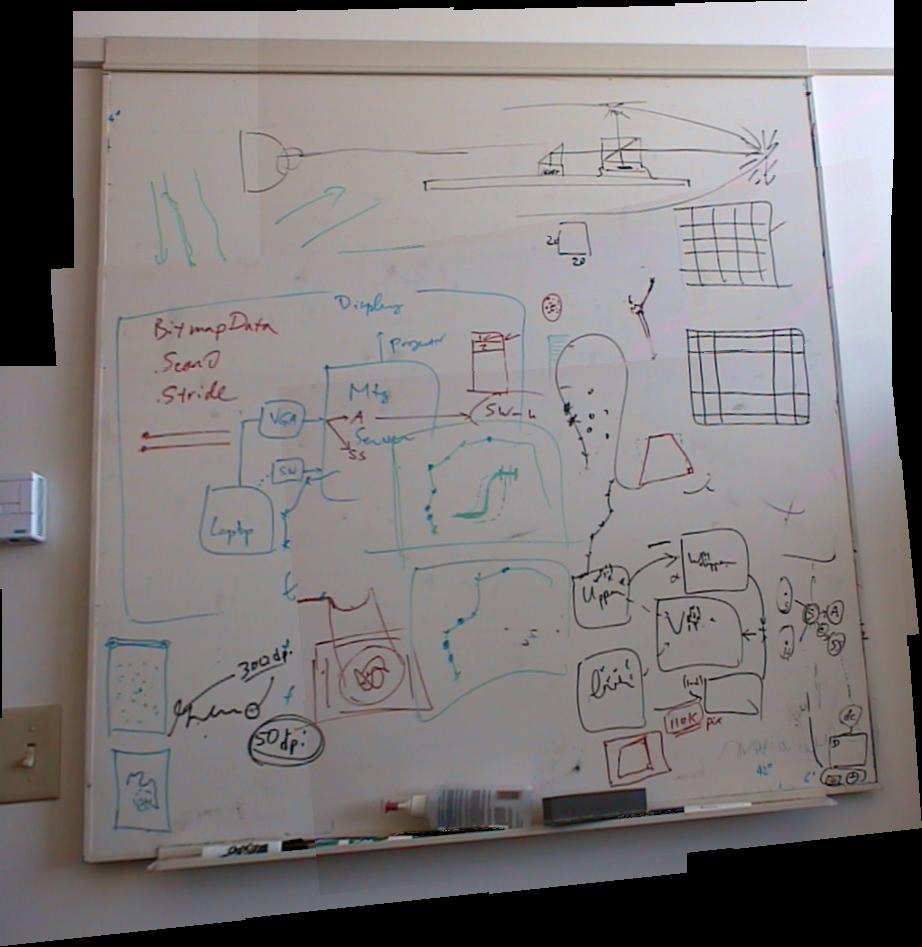
\includegraphics[width=\textwidth]{images/zhang_2004_1}
  \end{subfigure}
  \begin{subfigure}[b]{0.3\textwidth}
    \centering
    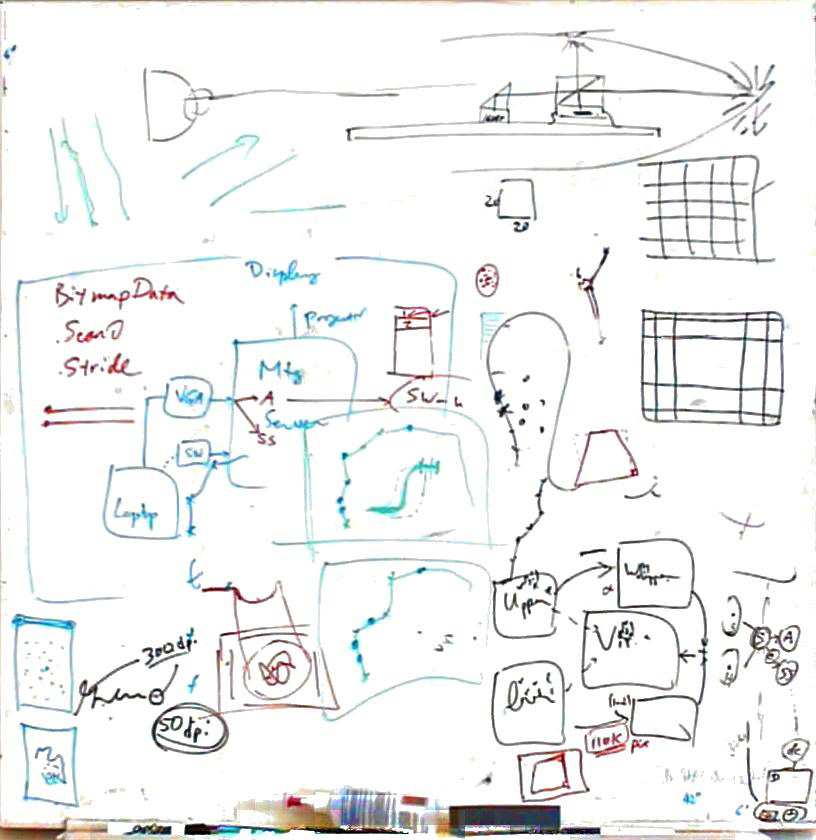
\includegraphics[width=\textwidth]{images/zhang_2004_2}
  \end{subfigure}
  \label{fig:zhang:2004}
  \caption{Демонстрація роботи алгоритму інженерів з Microsoft}
\end{figure}

Також автори реалізували склейку зображень дошки зроблених з різних
перспектив за допомогою гомографії. Гарна якість оцифрування дошки
досягається насамперед тим, що вона має білий колір, що в свою чергу
накладає обмеження для використання технології з дошками зеленого чи
чорного кольорів.
У наступній свої роботі \cite{zhang:2007} ціж самі автори побудували
систему, яка в реальному часі обробляє відеозапис, видаляє людину біля 
дошки за допомогою часової медіани, але в даному випадку немає 
панорамного склеювання знімків. Головна ідея роботи була зробити 
програму для телеконференсій.

\subsection{Автоматичне сканування дошки}

Автори даної роботи \cite{wienecke} створили програму яка переводить написи на білій 
дошці у цифрові. Вони реалізували локалізацію тексту та подальшу 
його обробку. Дана технологія не передбачає перекривання викладачем написів
або дошку іншого кольору відмінного від білого.

\begin{figure}[h]
  \centering
  \begin{subfigure}[b]{0.3\textwidth}
    \centering
    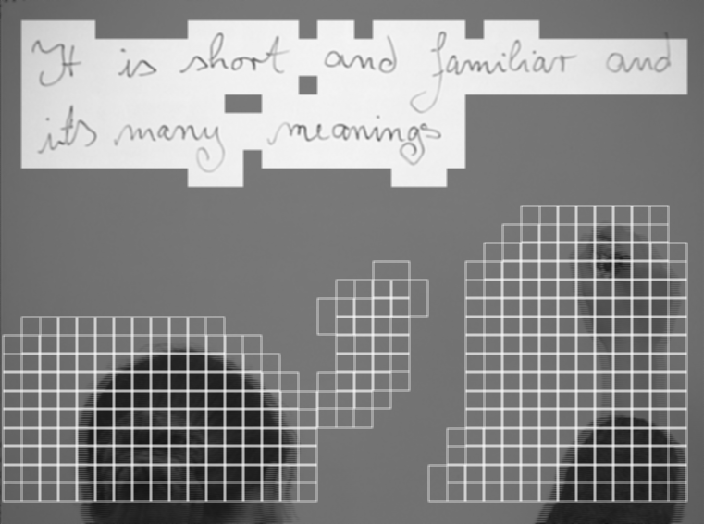
\includegraphics[width=\textwidth]{images/wienecke_1}
  \end{subfigure}
  \begin{subfigure}[b]{0.3\textwidth}
    \centering
    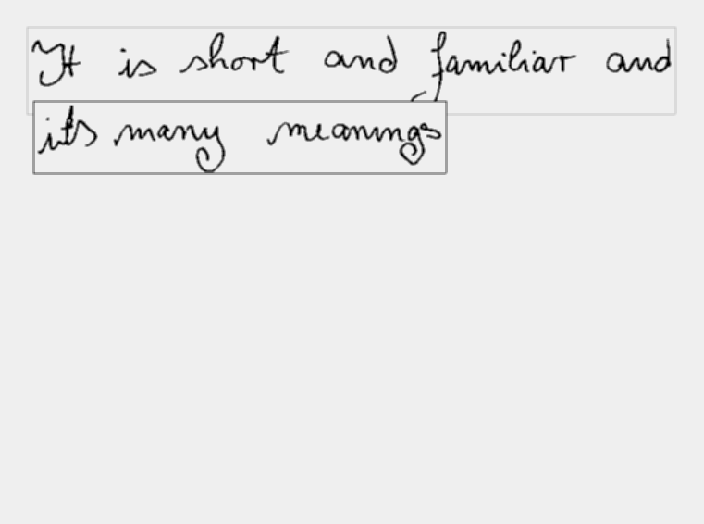
\includegraphics[width=\textwidth]{images/wienecke_2}
  \end{subfigure}
  \label{fig:wienecke}
  \caption{Демонстрація роботи сканування дошки}
\end{figure}

Можна помітити, що як і в попередній роботі гарна якість виокремлення написів
досягається тим що дошка білого кольору.

\subsection{Відстежування об'єкту та віднімання фону від Стенфорду}

У 2012 році науковці зі Стенфордського університету \textit{Alex Gonzalez, 
Bongsoo Suh, Eun Soo Choi} представили технологію \cite{sah} локалізацію дошки
(навіть такої яка розділена на частини), відстеження викладача та його
подальше прибирання. Алгоритм також може працювати з різними кольрами
дошок. Для прибирання викладача і всіх рухомих об'єктів автори також 
використали тимчасову медіану.

Дана програма не працює в реальному часі, оскільки всі операції над кадрами
відео займають тривалий час, не кажучи вже, що відео перед обробкою 
піддають компресії.

\begin{figure}[h]
  \centering
  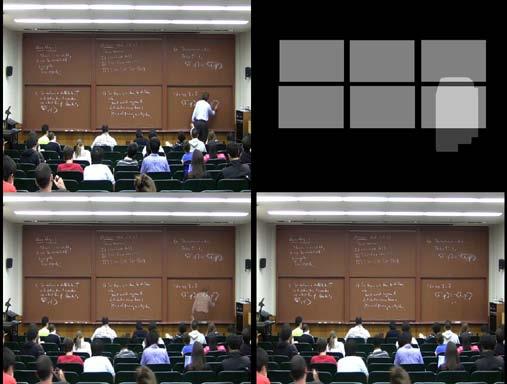
\includegraphics[width=0.5\textwidth]{images/sah}
  \caption{Приклад роботи авторів Стенфорду}
  \label{fig:sah}
\end{figure}

Головною особливістю даної роботи є те, що  алгоритм автоматично локалізує 
різну кількість дошок. Однак варто відмітити, що тестування відбувалось на
відеолекціях де камера знімає всю дошку і не рухається за викладачем. Тим більше
якість отриманих написів теж погана.

\subsection{Виокремлення написів дошки від Тайванського університету}

У 2014 році науковці із Тайванського університету представили свій аналог \cite{yeh} 
алгоритму по оцифровуванні дошки. Для видалення викладача автори застосували 
алгоритм кластеризації K-means. Для отримання бінаризованих написів з дошки 
використана адаптивне вирівнювання '(яке не ясно)'. Варто відмітити гарну
якість власного методу знешумлення.

\begin{figure}[h]
  \centering
  \begin{subfigure}[b]{0.3\textwidth}
    \centering
    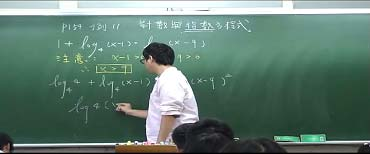
\includegraphics[width=\textwidth]{images/yeh_1}
  \end{subfigure}
  \begin{subfigure}[b]{0.3\textwidth}
    \centering
    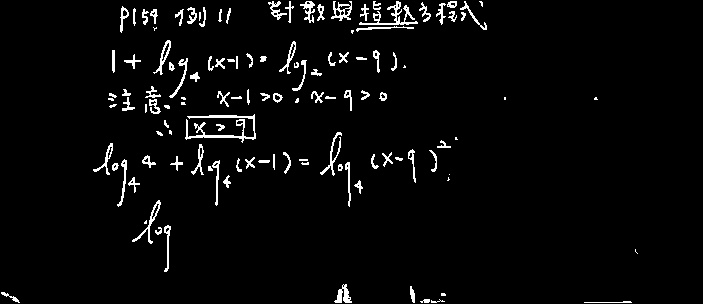
\includegraphics[width=\textwidth]{images/yeh_2}
  \end{subfigure}
  \label{fig:yeh}
  \caption{Демонстрація роботи сканування дошки}
\end{figure}

Автори не представили швидкість обробки всього відео. Щоб отримати якісну сегментацію
дошки та викладача потрібно, щоб кадр містив тільки викладача, причому щоб одяг викладача
був сильно відмінним від кольору дошки. Це потрібно для коректної роботи K-means.
Тобто нема гарантії, що якийсь рухомий об'єкт не стане  дошкою під час класифікації.

\subsection{Сучасна робота}

На даний момент найсучаснішою повною технологією \cite{davila:2017}, яка оцифровує дошку є робота
науковців з університету Рочестер. Автори \textit{Kenny Davila та Richard Zanibbi}
використали просторовий темпоралььний індекс для викремлення написів і викладача.
Відбувається видалення не самого викладача,  а його контурів, після бінаризації картинки.
Варто відмітити, що і тут камера має бути нерухомою.

\begin{figure}[h]
  \centering
  \begin{subfigure}[b]{0.3\textwidth}
    \centering
    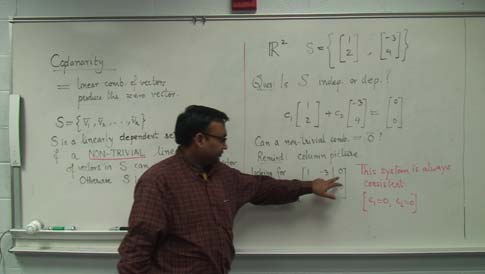
\includegraphics[width=\textwidth]{images/davila_2017_1}
  \end{subfigure}
  \begin{subfigure}[b]{0.3\textwidth}
    \centering
    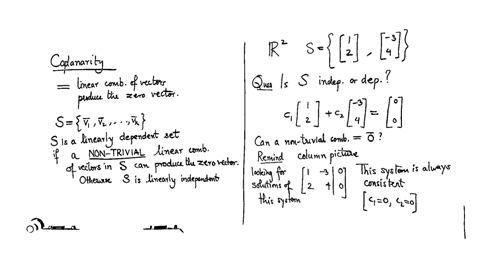
\includegraphics[width=\textwidth]{images/davila_2017_2}
  \end{subfigure}
  \label{fig:davila:2017}
  \caption{Демонстрація роботи сканування дошки}
\end{figure}

Пізніше ціж автори створили повністю згорткову нейронну мережу \cite{davila:2021}
для обробки написів дошки.Дана нейронна мережа LectureNet досить добре бінаризує написи з дошки.

\begin{figure}[h]
  \centering
  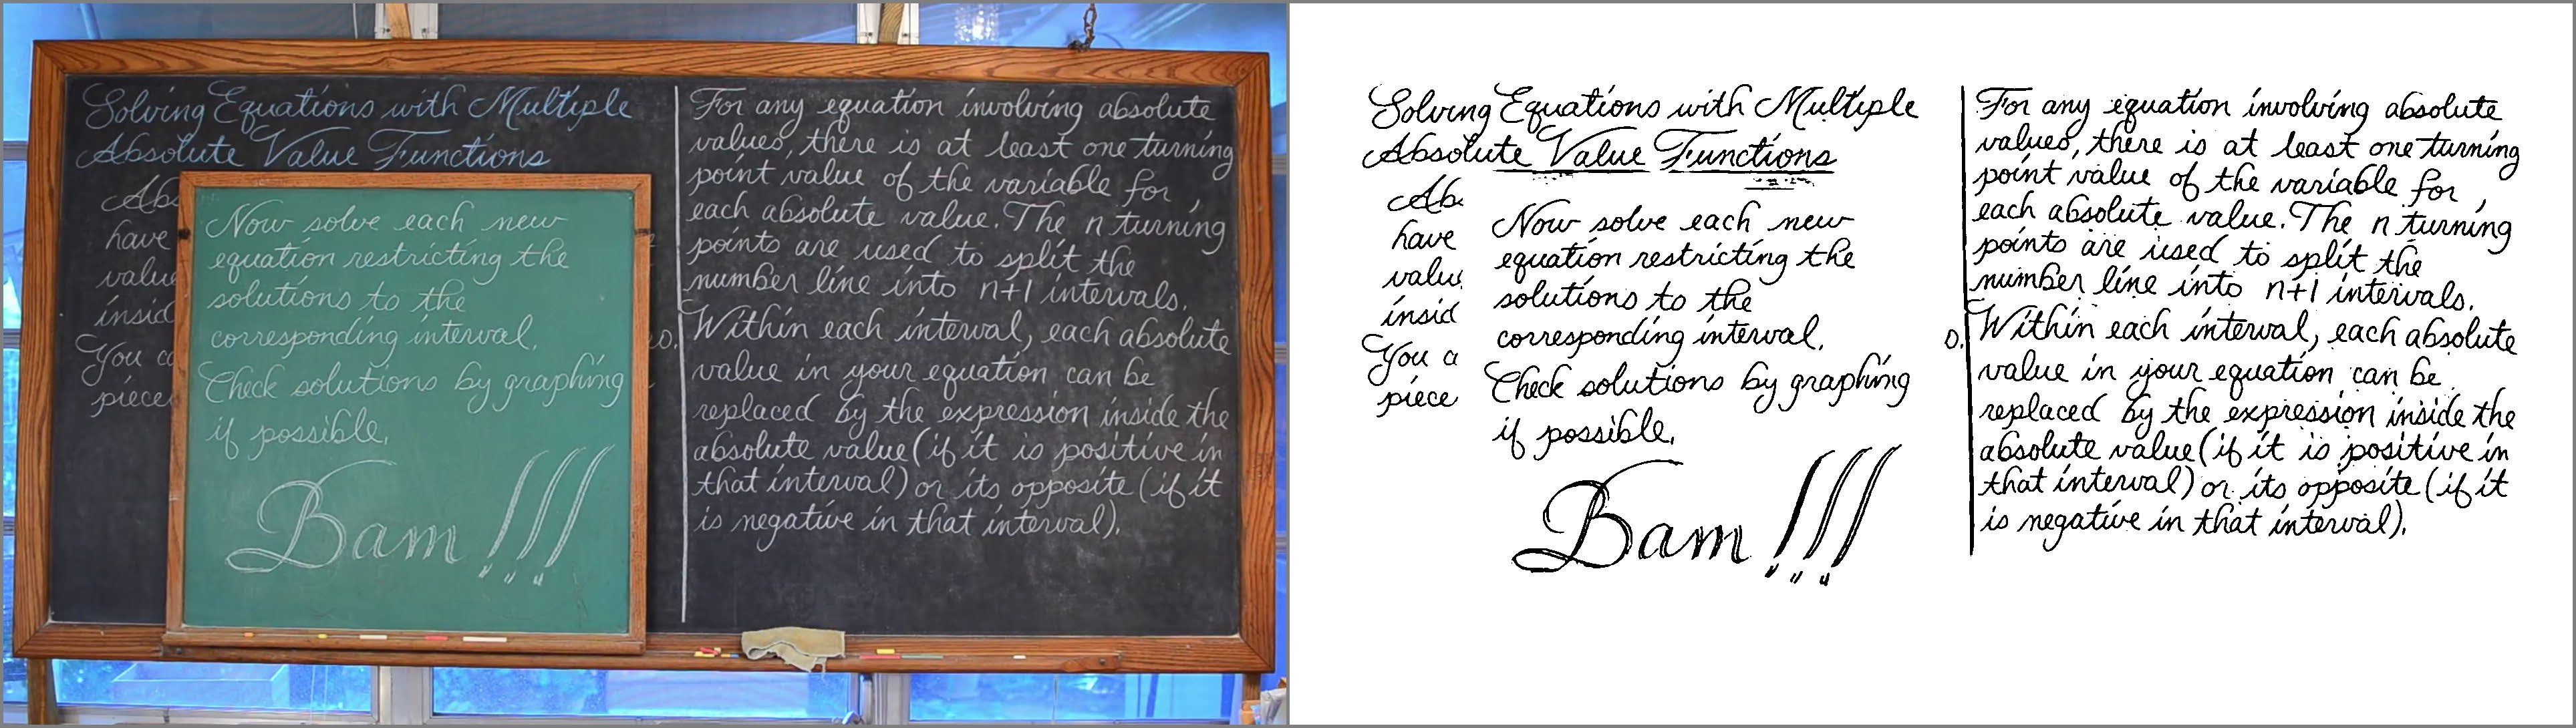
\includegraphics[width=0.5\textwidth]{images/davila_2021}
  \caption{Приклад роботи авторів з Рочестер}
  \label{fig:davila:2021}
\end{figure}


\subsection{Кінцевий аналіз робіт}

Як ми бачимо, всі вищеописані алгоритми є частковими (тобто не повністю вирішують всі проблеми
з оцифруванням дошки): якісь методи опрацьовують тільки написи з дошки, 
при чому досить непогано; якісь роблять панорамні знімки тільки з фотографій дошки.

Спільними елементами вищеописаних алгоритмів-аналогів є використання 
темпорального медіанного фільтру для видалення рухомих об'єктів.
У даній роботі даний метод теж має місце, але вже для знешумлення
вихідних слайдів, а не видалення лектора з відео.

Найбільшими недоліками всіх аналогів є час обробки відео. Більшість технологій
тестувались на відео поганої якості, наприклад 240р - 720р. 

Також жоден метод не пропонує створювати панорамні знімки по мірі руху камери під
час зйомки.і 